% Options for packages loaded elsewhere
\PassOptionsToPackage{unicode}{hyperref}
\PassOptionsToPackage{hyphens}{url}
%
\documentclass[
]{article}
\usepackage{amsmath,amssymb}
\usepackage{iftex}
\ifPDFTeX
  \usepackage[T1]{fontenc}
  \usepackage[utf8]{inputenc}
  \usepackage{textcomp} % provide euro and other symbols
\else % if luatex or xetex
  \usepackage{unicode-math} % this also loads fontspec
  \defaultfontfeatures{Scale=MatchLowercase}
  \defaultfontfeatures[\rmfamily]{Ligatures=TeX,Scale=1}
\fi
\usepackage{lmodern}
\ifPDFTeX\else
  % xetex/luatex font selection
\fi
% Use upquote if available, for straight quotes in verbatim environments
\IfFileExists{upquote.sty}{\usepackage{upquote}}{}
\IfFileExists{microtype.sty}{% use microtype if available
  \usepackage[]{microtype}
  \UseMicrotypeSet[protrusion]{basicmath} % disable protrusion for tt fonts
}{}
\makeatletter
\@ifundefined{KOMAClassName}{% if non-KOMA class
  \IfFileExists{parskip.sty}{%
    \usepackage{parskip}
  }{% else
    \setlength{\parindent}{0pt}
    \setlength{\parskip}{6pt plus 2pt minus 1pt}}
}{% if KOMA class
  \KOMAoptions{parskip=half}}
\makeatother
\usepackage{xcolor}
\usepackage[margin=1in]{geometry}
\usepackage{color}
\usepackage{fancyvrb}
\newcommand{\VerbBar}{|}
\newcommand{\VERB}{\Verb[commandchars=\\\{\}]}
\DefineVerbatimEnvironment{Highlighting}{Verbatim}{commandchars=\\\{\}}
% Add ',fontsize=\small' for more characters per line
\usepackage{framed}
\definecolor{shadecolor}{RGB}{248,248,248}
\newenvironment{Shaded}{\begin{snugshade}}{\end{snugshade}}
\newcommand{\AlertTok}[1]{\textcolor[rgb]{0.94,0.16,0.16}{#1}}
\newcommand{\AnnotationTok}[1]{\textcolor[rgb]{0.56,0.35,0.01}{\textbf{\textit{#1}}}}
\newcommand{\AttributeTok}[1]{\textcolor[rgb]{0.13,0.29,0.53}{#1}}
\newcommand{\BaseNTok}[1]{\textcolor[rgb]{0.00,0.00,0.81}{#1}}
\newcommand{\BuiltInTok}[1]{#1}
\newcommand{\CharTok}[1]{\textcolor[rgb]{0.31,0.60,0.02}{#1}}
\newcommand{\CommentTok}[1]{\textcolor[rgb]{0.56,0.35,0.01}{\textit{#1}}}
\newcommand{\CommentVarTok}[1]{\textcolor[rgb]{0.56,0.35,0.01}{\textbf{\textit{#1}}}}
\newcommand{\ConstantTok}[1]{\textcolor[rgb]{0.56,0.35,0.01}{#1}}
\newcommand{\ControlFlowTok}[1]{\textcolor[rgb]{0.13,0.29,0.53}{\textbf{#1}}}
\newcommand{\DataTypeTok}[1]{\textcolor[rgb]{0.13,0.29,0.53}{#1}}
\newcommand{\DecValTok}[1]{\textcolor[rgb]{0.00,0.00,0.81}{#1}}
\newcommand{\DocumentationTok}[1]{\textcolor[rgb]{0.56,0.35,0.01}{\textbf{\textit{#1}}}}
\newcommand{\ErrorTok}[1]{\textcolor[rgb]{0.64,0.00,0.00}{\textbf{#1}}}
\newcommand{\ExtensionTok}[1]{#1}
\newcommand{\FloatTok}[1]{\textcolor[rgb]{0.00,0.00,0.81}{#1}}
\newcommand{\FunctionTok}[1]{\textcolor[rgb]{0.13,0.29,0.53}{\textbf{#1}}}
\newcommand{\ImportTok}[1]{#1}
\newcommand{\InformationTok}[1]{\textcolor[rgb]{0.56,0.35,0.01}{\textbf{\textit{#1}}}}
\newcommand{\KeywordTok}[1]{\textcolor[rgb]{0.13,0.29,0.53}{\textbf{#1}}}
\newcommand{\NormalTok}[1]{#1}
\newcommand{\OperatorTok}[1]{\textcolor[rgb]{0.81,0.36,0.00}{\textbf{#1}}}
\newcommand{\OtherTok}[1]{\textcolor[rgb]{0.56,0.35,0.01}{#1}}
\newcommand{\PreprocessorTok}[1]{\textcolor[rgb]{0.56,0.35,0.01}{\textit{#1}}}
\newcommand{\RegionMarkerTok}[1]{#1}
\newcommand{\SpecialCharTok}[1]{\textcolor[rgb]{0.81,0.36,0.00}{\textbf{#1}}}
\newcommand{\SpecialStringTok}[1]{\textcolor[rgb]{0.31,0.60,0.02}{#1}}
\newcommand{\StringTok}[1]{\textcolor[rgb]{0.31,0.60,0.02}{#1}}
\newcommand{\VariableTok}[1]{\textcolor[rgb]{0.00,0.00,0.00}{#1}}
\newcommand{\VerbatimStringTok}[1]{\textcolor[rgb]{0.31,0.60,0.02}{#1}}
\newcommand{\WarningTok}[1]{\textcolor[rgb]{0.56,0.35,0.01}{\textbf{\textit{#1}}}}
\usepackage{graphicx}
\makeatletter
\def\maxwidth{\ifdim\Gin@nat@width>\linewidth\linewidth\else\Gin@nat@width\fi}
\def\maxheight{\ifdim\Gin@nat@height>\textheight\textheight\else\Gin@nat@height\fi}
\makeatother
% Scale images if necessary, so that they will not overflow the page
% margins by default, and it is still possible to overwrite the defaults
% using explicit options in \includegraphics[width, height, ...]{}
\setkeys{Gin}{width=\maxwidth,height=\maxheight,keepaspectratio}
% Set default figure placement to htbp
\makeatletter
\def\fps@figure{htbp}
\makeatother
\setlength{\emergencystretch}{3em} % prevent overfull lines
\providecommand{\tightlist}{%
  \setlength{\itemsep}{0pt}\setlength{\parskip}{0pt}}
\setcounter{secnumdepth}{-\maxdimen} % remove section numbering
\ifLuaTeX
  \usepackage{selnolig}  % disable illegal ligatures
\fi
\usepackage{bookmark}
\IfFileExists{xurl.sty}{\usepackage{xurl}}{} % add URL line breaks if available
\urlstyle{same}
\hypersetup{
  pdftitle={Práctica dirigida 10},
  hidelinks,
  pdfcreator={LaTeX via pandoc}}

\title{Práctica dirigida 10}
\author{}
\date{\vspace{-2.5em}}

\begin{document}
\maketitle

{
\setcounter{tocdepth}{1}
\tableofcontents
}

\includegraphics[width=0.3\linewidth]{logoPUCP}

\section{\texorpdfstring{\textbf{Regresión linea
múltiple}}{Regresión linea múltiple}}\label{regresiuxf3n-linea-muxfaltiple}

Hasta el momento, nos hemos encontrado en el campo del análisis
bivariado. Sin embargo, en el mundo social, difícilmente se pueden
explicar los fenómenos de interés con una sola variable. Incluso si nos
interesa evaluar el efecto de un a variable en específico sobre un
fenómeno de estudio, hay muchos otros factores que podrían influir en
aquello que nos interesa explorar. Por ello, necesitamos recurrir al
\textbf{análisis multivariado} y conocer el concepto de \textbf{control
estadístico}.

El control estadístico nos permite aislar el efecto de otras variables.
La idea es:

\begin{itemize}
\item
  Evaluar si la asociación entre X e Y permanece si se remueve el efecto
  de otra variable, es decir, si se controla por una tercera variable.
\item
  Se analiza la relación entre X e Y para valores similares o iguales de
  una variable Z. De esta manera se elimina la influencia de Z en la
  relación entre X e Y. Lo anterior nos ayuda a acercarnos a una
  interpretación causar X -\textgreater{} Y.
\item
  Si la relación entre X e Y desaparece cuando se controla por Z, se
  dice que la relación era espúrea. En otras palabras, la relación
  dependendia de la influencia de Z y no de una conexión directa entre X
  e Y.
\end{itemize}

Sobre la regresión lineal múltiple:

\begin{center}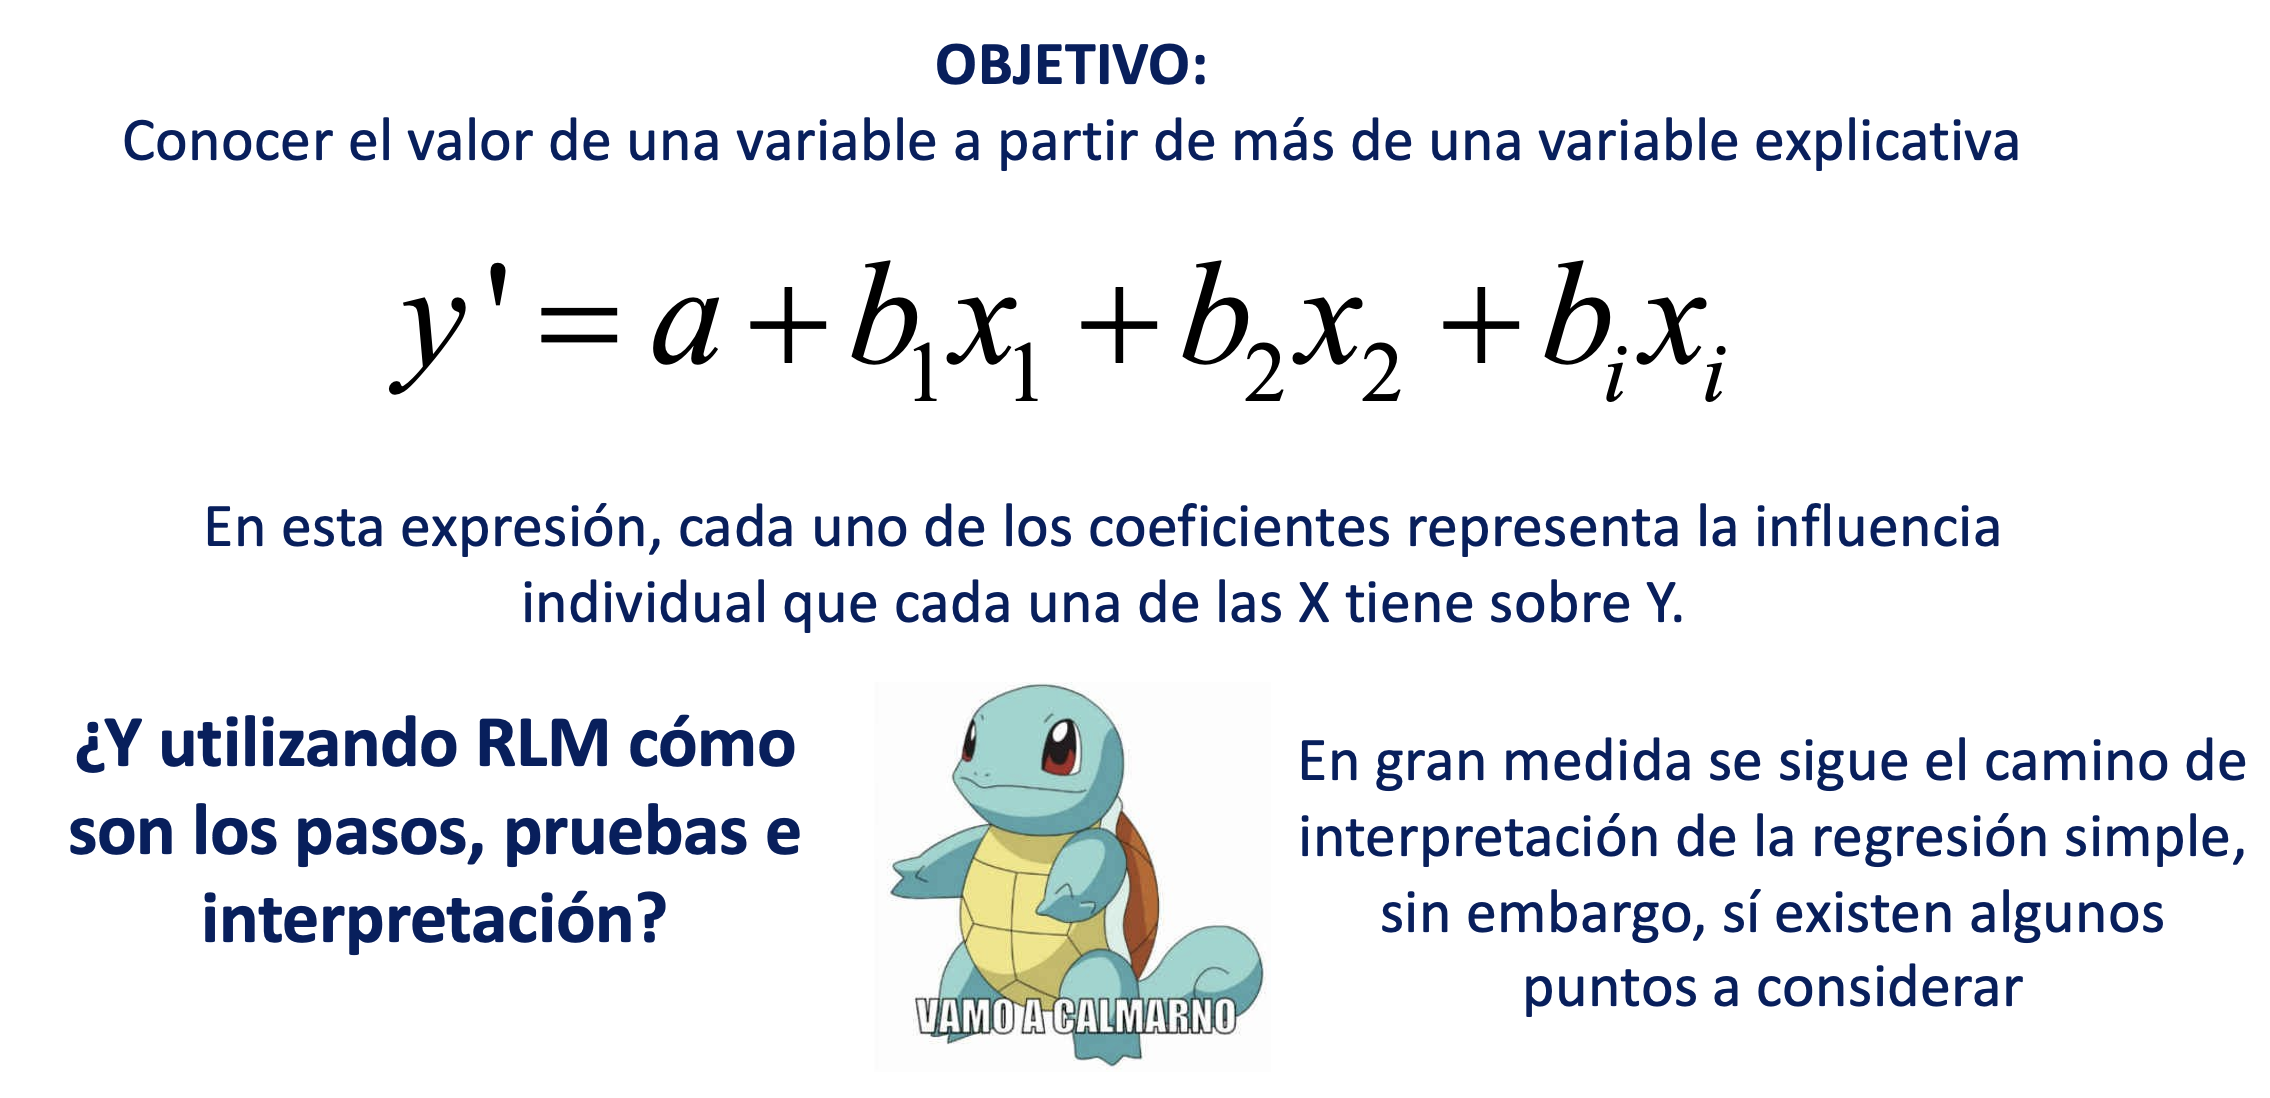
\includegraphics[width=1\linewidth]{pd12_diap1} \end{center}

\begin{center}\rule{0.5\linewidth}{0.5pt}\end{center}

Seguiremos los siguientes pasos para el análisis:

\begin{center}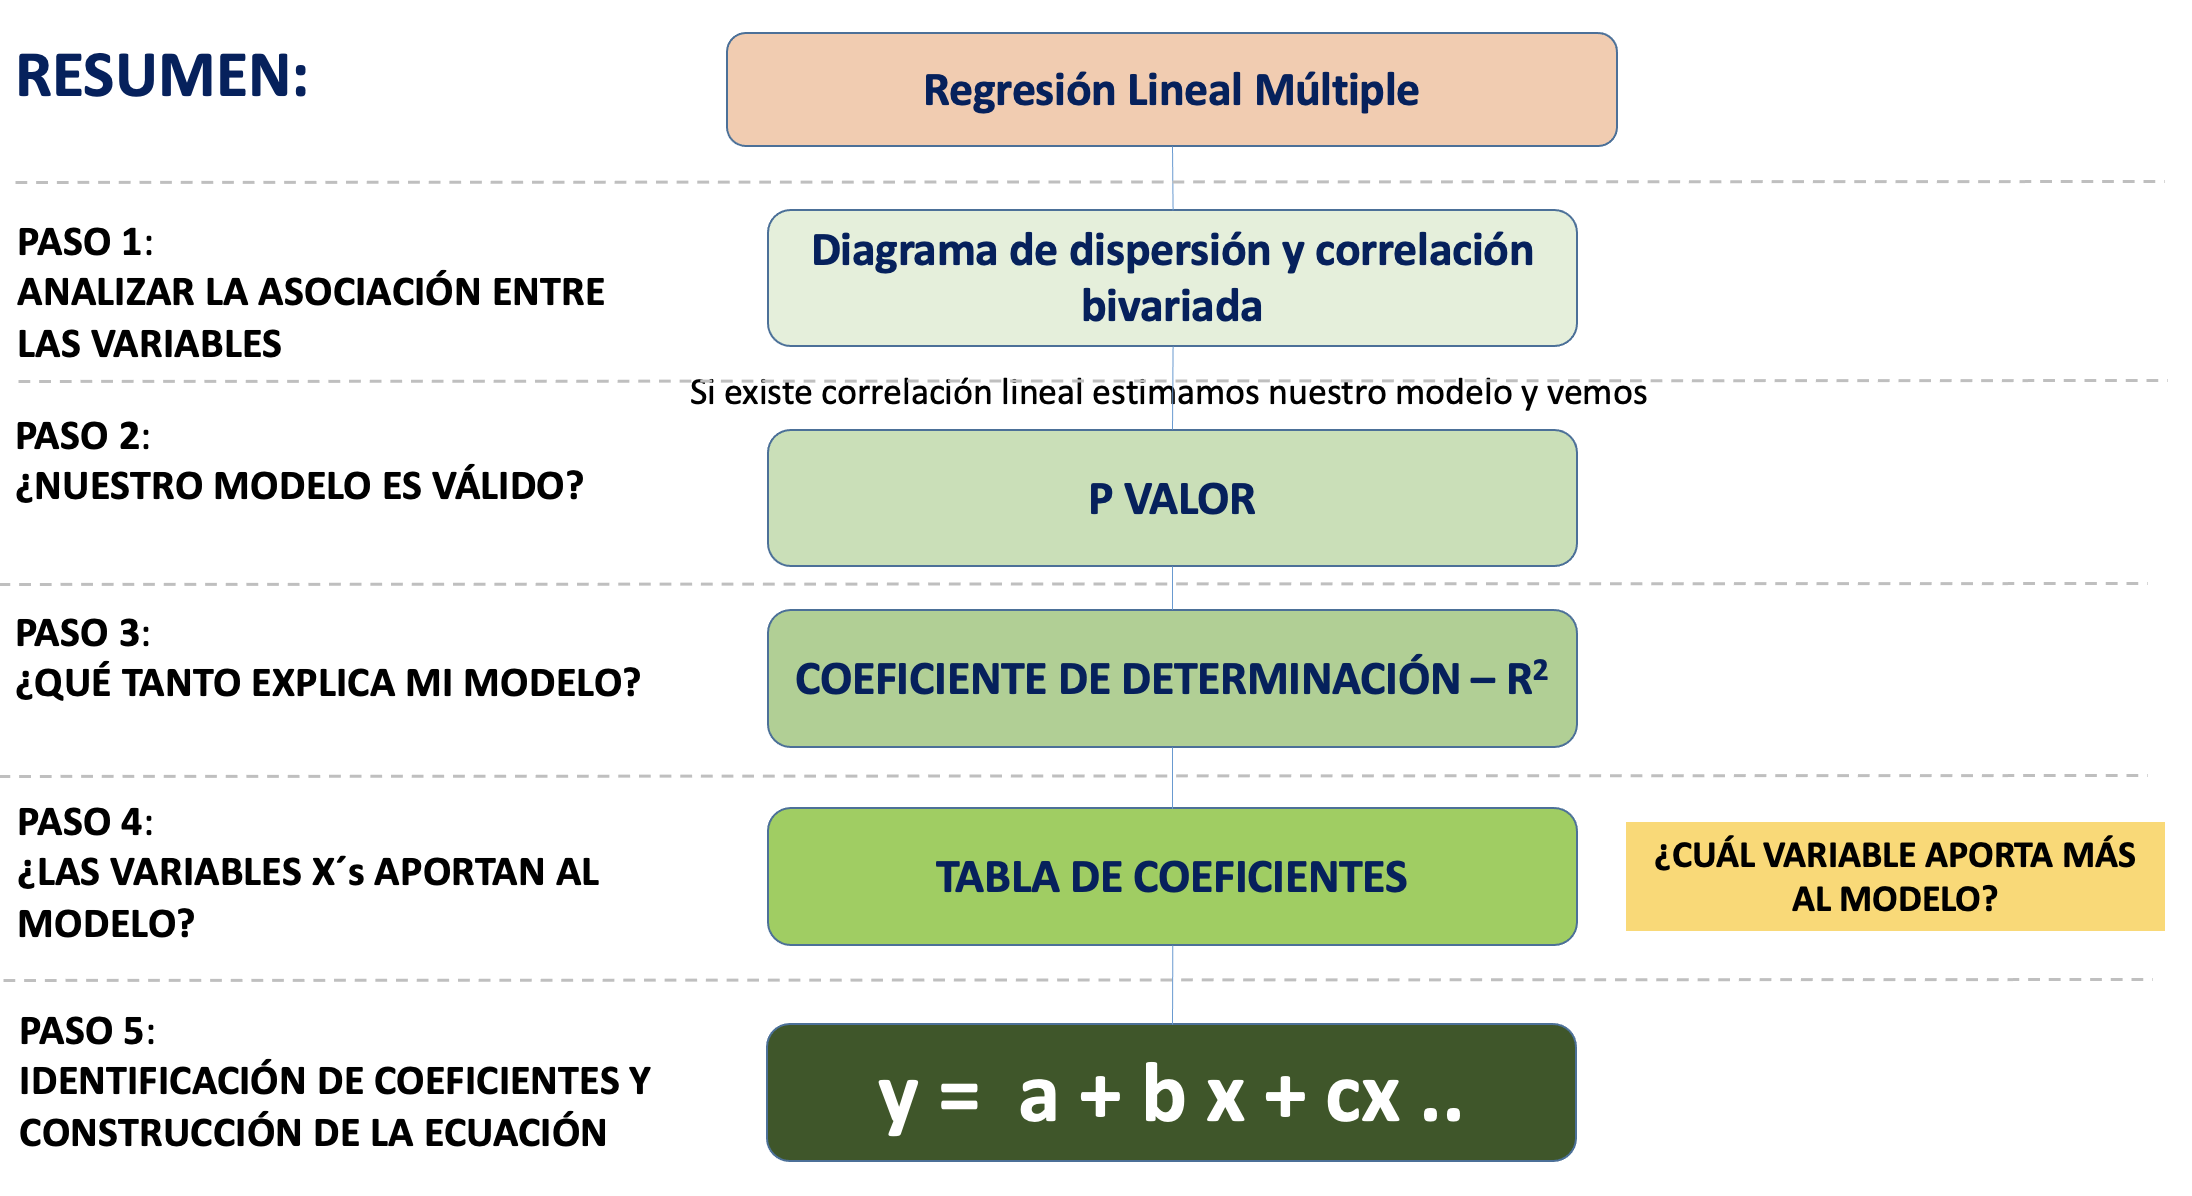
\includegraphics[width=1\linewidth]{pd12_diap2} \end{center}

\section{Aplicación práctica}\label{aplicaciuxf3n-pruxe1ctica}

\subsection{\texorpdfstring{\textbf{Factores que determinan el acceso a
la información en los
Estados}}{Factores que determinan el acceso a la información en los Estados}}\label{factores-que-determinan-el-acceso-a-la-informaciuxf3n-en-los-estados}

El acceso a la información es fundamental para el funcionamiento de
cualquier Estado democrático, ya que promueve la transparencia, la
responsabilidad y la participación ciudadana.

Para poder realizar el análisis se han revisado las siguientes fuentes:

\textbf{Digital Access Index} El Índice de Acceso Digital es utilizado
para medir y evaluar el nivel de acceso a las tecnologías digitales y a
internet. Proporciona una medida de hasta qué punto las personas y las
comunidades pueden utilizar y beneficiarse de las tecnologías digitales.

\textbf{Egov-index} El Índice de Gobierno Electrónico es una medida que
evalúa el nivel de desarrollo y adopción de tecnologías de la
información y la comunicación (TIC) en el sector público. Este índice se
utiliza para medir la capacidad de los gobiernos para proporcionar
servicios en línea, promover la participación ciudadana y utilizar las
TIC de manera efectiva en la gestión gubernamental.

\textbf{Democracy Index} El Índice de Democracia es un índice que mide
el estado de la democracia en países de todo el mundo. Es elaborado por
The Economist (EIU) y evalúa el funcionamiento de los procesos e
instituciones democráticas.

A partir de la información recolectada se ha creado una base de datos
llamada Egov.

\begin{center}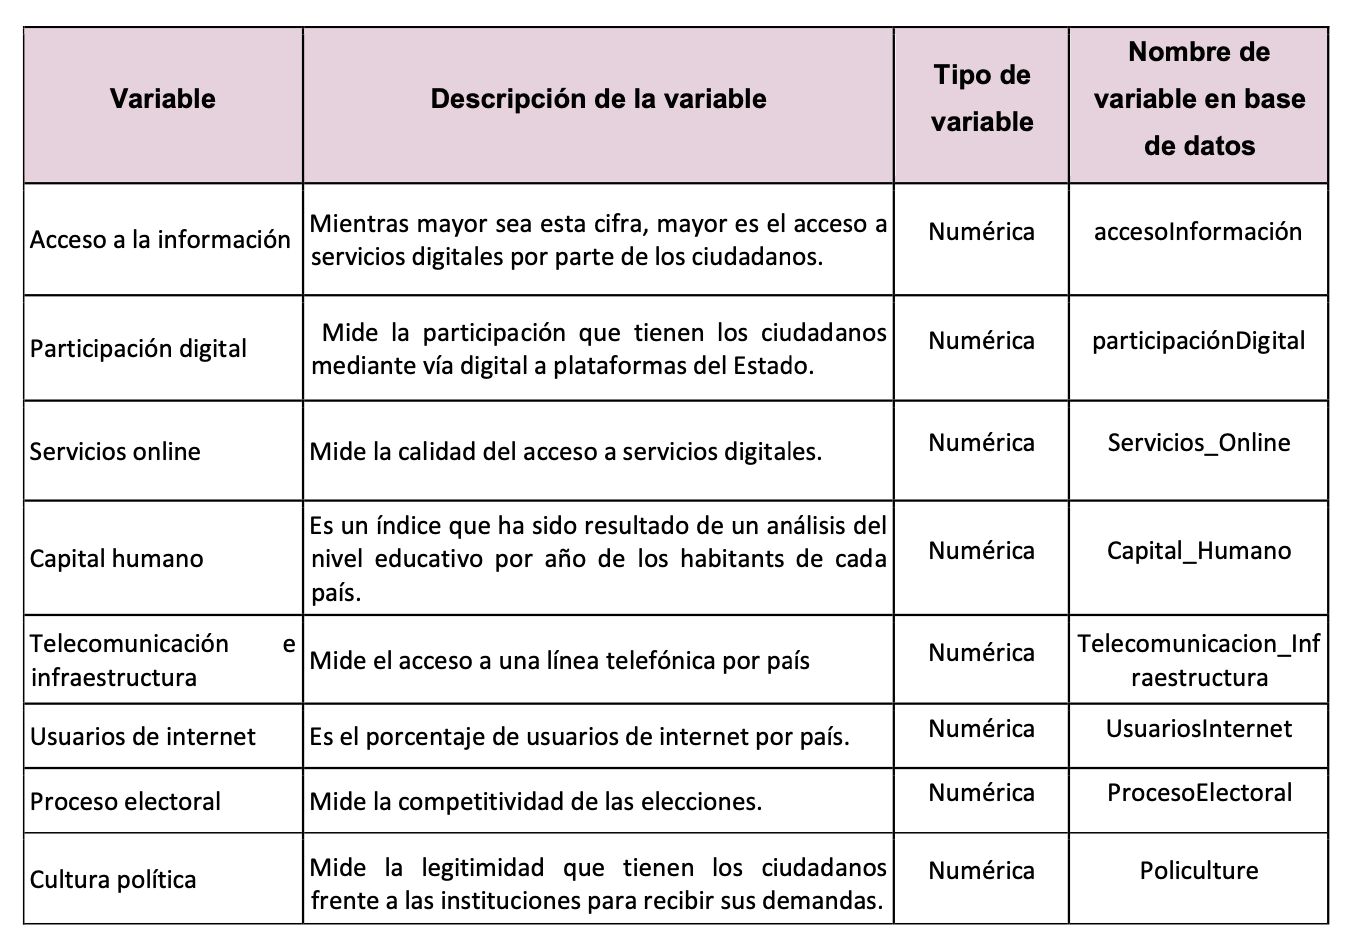
\includegraphics[width=0.8\linewidth]{PD12_diccionarioEgov} \end{center}

\begin{Shaded}
\begin{Highlighting}[]
\FunctionTok{library}\NormalTok{(rio)}
\NormalTok{Egov}\OtherTok{=}\FunctionTok{import}\NormalTok{(}\StringTok{"EGov.xlsx"}\NormalTok{)}
\FunctionTok{names}\NormalTok{(Egov)}
\end{Highlighting}
\end{Shaded}

\begin{verbatim}
## [1] "pais"                             "participaciónDigital"            
## [3] "Servicios_Online"                 "Capital_Humano"                  
## [5] "Telecommunicacion_Infrastructura" "ProcesoElectoral"                
## [7] "Policulture"                      "accesoInformacion"               
## [9] "UsuariosInternet"
\end{verbatim}

\textbf{No olviden el análisis descriptivo antes de hacer los modelos.}

\subsection{\texorpdfstring{\textbf{Modelo
1}}{Modelo 1}}\label{modelo-1}

\begin{Shaded}
\begin{Highlighting}[]
\FunctionTok{library}\NormalTok{(tidyverse)}

\NormalTok{modelo1 }\OtherTok{=} \FunctionTok{lm}\NormalTok{(accesoInformacion }\SpecialCharTok{\textasciitilde{}}\NormalTok{participaciónDigital}\SpecialCharTok{+}\NormalTok{Servicios\_Online}\SpecialCharTok{+}\NormalTok{Capital\_Humano  }\SpecialCharTok{+}\NormalTok{Telecommunicacion\_Infrastructura}\SpecialCharTok{+}\NormalTok{ProcesoElectoral}\SpecialCharTok{+}\NormalTok{ Policulture }\SpecialCharTok{+}\NormalTok{UsuariosInternet ,}\AttributeTok{data=}\NormalTok{Egov)}
\FunctionTok{summary}\NormalTok{(modelo1)}
\end{Highlighting}
\end{Shaded}

\begin{verbatim}
## 
## Call:
## lm(formula = accesoInformacion ~ participaciónDigital + Servicios_Online + 
##     Capital_Humano + Telecommunicacion_Infrastructura + ProcesoElectoral + 
##     Policulture + UsuariosInternet, data = Egov)
## 
## Residuals:
##       Min        1Q    Median        3Q       Max 
## -0.204651 -0.033054  0.002505  0.032268  0.116256 
## 
## Coefficients:
##                                    Estimate Std. Error t value Pr(>|t|)    
## (Intercept)                      -0.1208398  0.0263792  -4.581 1.13e-05 ***
## participaciónDigital             -0.0788712  0.0914304  -0.863  0.39004    
## Servicios_Online                  0.0809775  0.0948445   0.854  0.39491    
## Capital_Humano                    0.2968634  0.0555961   5.340 4.43e-07 ***
## Telecommunicacion_Infrastructura  0.3561180  0.0782623   4.550 1.28e-05 ***
## ProcesoElectoral                  0.0075843  0.0019182   3.954  0.00013 ***
## Policulture                       0.0139957  0.0043417   3.224  0.00163 ** 
## UsuariosInternet                  0.0015629  0.0006815   2.293  0.02355 *  
## ---
## Signif. codes:  0 '***' 0.001 '**' 0.01 '*' 0.05 '.' 0.1 ' ' 1
## 
## Residual standard error: 0.06194 on 121 degrees of freedom
## Multiple R-squared:  0.926,  Adjusted R-squared:  0.9217 
## F-statistic: 216.3 on 7 and 121 DF,  p-value: < 2.2e-16
\end{verbatim}

\subsection{\texorpdfstring{\textbf{Interpretamos
😎}}{Interpretamos 😎}}\label{interpretamos}

\subsubsection{\texorpdfstring{\textbf{¿El modelo es
válido?}}{¿El modelo es válido?}}\label{el-modelo-es-vuxe1lido}

Establezcamos nuestras hipótesis:

\begin{itemize}
\tightlist
\item
  H0: El modelo de regresión no es válido
\item
  H1: El modelo de regresión es válido (las variables independientes
  aportan al modelo)
\end{itemize}

Luego nos fijamos en el \textbf{p-value} Como el p valor es \textless{}
2.2e-16 entonces podemos afirmar que hay suficiente evidencia para
rechazar la H0, por lo que concluimos que el modelo es válido como
modelo de predicción.

\subsubsection{\texorpdfstring{\textbf{¿Qué tanto explica el
modelo?}}{¿Qué tanto explica el modelo?}}\label{quuxe9-tanto-explica-el-modelo}

Observamos el \textbf{R2 ajustado}.

Analizar cuánto de la variabilidad de la variable dependiente (y) es
explicada por las variables independientes elegidas, para ello revisamos
el R2 (Adjusted R-squared, por ser un modelo lineal múltiple).

En nuestro modelo, este arrojó el valor de 0.9217, por lo que podemos
concluir que el modelo explica aproximadamente el 92.2\% (0.9217*100) de
la variabilidad en el acceso a la información (variable dependiente). En
otras palabras, este valor alto de R cuadrado ajustado indica que el
modelo se ajusta muy bien a los datos y hace un buen trabajo al explicar
la relación entre las variables independientes y la variable
dependiente. Sin embargo, el valor del R cuadrado ajustado no te dice
nada sobre la significancia estadística de las variables individuales,
ni sobre la causalidad. Por ello analizaremos también las variables de
forma independiente en el siguiente paso.

\emph{Recordemos que el R cuadrado puede tomar valores entre 0 y 1. Un R
cuadrado de 1 indica que el modelo explica toda la variabilidad de la
variable Y. Un R cuadrado de 0 indica que el modelo no explica nada de
la variabilidad de la variable Y.}

\subsubsection{\texorpdfstring{\textbf{¿Las variables aportan al
modelo?}}{¿Las variables aportan al modelo?}}\label{las-variables-aportan-al-modelo}

Revisamos \textbf{p-value} por cada variable independiente.

\begin{itemize}
\tightlist
\item
  Esperamos obtener un p-value \textless0.05.
\item
  Nos damos cuenta que \emph{no todas} las variables independientes
  tienen un p-value \textless0.05, es el caso de: participaciónDigital y
  Servicios\_Online
\end{itemize}

\subsubsection{\texorpdfstring{\textbf{¿Cuáles son los coeficientes de
la
ecuación?}}{¿Cuáles son los coeficientes de la ecuación?}}\label{cuuxe1les-son-los-coeficientes-de-la-ecuaciuxf3n}

Podemos obtener extraer los coeficientes del modelo:

\emph{No olvidar identificar el signo de cada coeficiente, este tendrá
repercusión en la ecuación y su futura aplicación}

\begin{Shaded}
\begin{Highlighting}[]
\NormalTok{modelo1}\SpecialCharTok{$}\NormalTok{coefficients}
\end{Highlighting}
\end{Shaded}

\begin{verbatim}
##                      (Intercept)             participaciónDigital 
##                     -0.120839771                     -0.078871158 
##                 Servicios_Online                   Capital_Humano 
##                      0.080977535                      0.296863439 
## Telecommunicacion_Infrastructura                 ProcesoElectoral 
##                      0.356118022                      0.007584279 
##                      Policulture                 UsuariosInternet 
##                      0.013995704                      0.001562898
\end{verbatim}

De esa manera puedo hallar la ecuación:

\[
Y = -0.12 + \text{participaciónDigital} \times (-0.078) + \text{Servicios\_Online} \times (0.080) + \text{Capital\_Humano} \times (0.29) + \text{Telecommunicacion\_Infrastructura} \times (0.35) + \text{ProcesoElectoral} \times (0.0075) + \text{Policulture} \times (0.013) + \text{UsuariosInternet} \times (0.0015)
\]

Es decir, se tienen las siguientes relaciones entre VD y las VI:

\begin{itemize}
\item
  Por cada unidad adicional de puntaje en participación digital, el
  índice de acceso a la información \textbf{disminuye en 0.078 puntos}
  (relación inversa).
\item
  Por cada unidad adicional de puntaje de servicios online, el índice de
  acceso a la información \textbf{aumenta en 0.08 puntos}. (relación
  directa).
\item
  Por cada unidad adicional de puntaje en Capital Humano, el índice de
  acceso a la información \textbf{aumenta en 0.08 puntos} (relación
  directa).
\item
  Por cada unidad adicional de puntaje de telecomunicaciones e
  infraestructura, el índice de acceso a la información \textbf{aumenta
  en 0.35 puntos}. (relación directa).
\item
  Por cada unidad adicional de puntaje de Procesos Electorales, el
  índice de acceso a la información \textbf{aumenta en 0.0075 puntos}.
  (relación directa).
\item
  Por cada unidad adicional de puntaje de Cultura política, el índice de
  acceso a la información \textbf{aumenta en 0.013 puntos}. (relación
  directa).
\item
  Por cada unidad adicional de puntaje de acceso de Usuarios a Internet,
  el índice de acceso a la información \textbf{aumenta en 0.0015
  puntos}. (relación directa).
\end{itemize}

\textbf{OJO: La ecuación de la recta debe incluir TODAS las variables
analizadas, tengan o no una influencia significativa en la VD.}

¿Qué sucede si retiro las variables independientes que no aportan al
modelo 1? Veamos un segundo modelo 👀 .

\subsection{\texorpdfstring{\textbf{Modelo
2}}{Modelo 2}}\label{modelo-2}

\begin{Shaded}
\begin{Highlighting}[]
\FunctionTok{library}\NormalTok{(dplyr)}
\FunctionTok{library}\NormalTok{(ggplot2)}

\NormalTok{modelo2 }\OtherTok{=} \FunctionTok{lm}\NormalTok{(accesoInformacion }\SpecialCharTok{\textasciitilde{}}\NormalTok{Capital\_Humano  }\SpecialCharTok{+}\NormalTok{Telecommunicacion\_Infrastructura}\SpecialCharTok{+}\NormalTok{ProcesoElectoral}\SpecialCharTok{+}\NormalTok{ Policulture }\SpecialCharTok{+}\NormalTok{UsuariosInternet   ,}\AttributeTok{data=}\NormalTok{Egov)}
\FunctionTok{summary}\NormalTok{(modelo2)}
\end{Highlighting}
\end{Shaded}

\begin{verbatim}
## 
## Call:
## lm(formula = accesoInformacion ~ Capital_Humano + Telecommunicacion_Infrastructura + 
##     ProcesoElectoral + Policulture + UsuariosInternet, data = Egov)
## 
## Residuals:
##       Min        1Q    Median        3Q       Max 
## -0.205352 -0.037077  0.002991  0.035621  0.111936 
## 
## Coefficients:
##                                    Estimate Std. Error t value Pr(>|t|)    
## (Intercept)                      -0.1220640  0.0262044  -4.658 8.15e-06 ***
## Capital_Humano                    0.2884448  0.0538523   5.356 4.02e-07 ***
## Telecommunicacion_Infrastructura  0.3513669  0.0774659   4.536 1.34e-05 ***
## ProcesoElectoral                  0.0075854  0.0018682   4.060 8.66e-05 ***
## Policulture                       0.0145801  0.0042686   3.416 0.000863 ***
## UsuariosInternet                  0.0016876  0.0006405   2.635 0.009498 ** 
## ---
## Signif. codes:  0 '***' 0.001 '**' 0.01 '*' 0.05 '.' 0.1 ' ' 1
## 
## Residual standard error: 0.06163 on 123 degrees of freedom
## Multiple R-squared:  0.9255, Adjusted R-squared:  0.9225 
## F-statistic: 305.8 on 5 and 123 DF,  p-value: < 2.2e-16
\end{verbatim}

\subsection{\texorpdfstring{\textbf{Interpretamos
😎}}{Interpretamos 😎}}\label{interpretamos-1}

\subsubsection{\texorpdfstring{\textbf{¿El modelo es
válido?}}{¿El modelo es válido?}}\label{el-modelo-es-vuxe1lido-1}

Establezcamos nuestras hipótesis:

\begin{itemize}
\tightlist
\item
  H0: El modelo de regresión no es válido
\item
  H1: El modelo de regresión es válido (las variables independientes
  aportan al modelo)
\end{itemize}

Luego nos fijamos en el \textbf{p-value} Como el p valor es \textless{}
2.2e-16 entonces podemos afirmar que hay suficiente evidencia para
rechazar la H0, por lo que concluimos que el modelo sí es válido como
modelo de predicción.

\subsubsection{\texorpdfstring{\textbf{¿Qué tanto explica el
modelo?}}{¿Qué tanto explica el modelo?}}\label{quuxe9-tanto-explica-el-modelo-1}

Observamos el \textbf{R2 ajustado}.

Analizar cuánto de la variabilidad de la variable dependiente (y) es
explicada por las variables independientes elegidas, para ello revisamos
el R2 (Adjusted R-squared).

En nuestro modelo, este arrojó el valor de 0.9225, por lo que podemos
concluir mi modelo explica aproximadamente el 92.25\% (0.9225*100) de la
variabilidad en el acceso a la información (variable dependiente). E

\subsubsection{\texorpdfstring{\textbf{¿Las variables aportan al
modelo?}}{¿Las variables aportan al modelo?}}\label{las-variables-aportan-al-modelo-1}

Revisamos \textbf{p-value} por cada variable independiente.

\begin{itemize}
\tightlist
\item
  Esperamos obtener un p-value \textless0.05.
\item
  \emph{Todas} las variables independientes aportan al modelo.
\end{itemize}

\subsubsection{\texorpdfstring{\textbf{¿Cuáles son los coeficientes de
la
ecuación?}}{¿Cuáles son los coeficientes de la ecuación?}}\label{cuuxe1les-son-los-coeficientes-de-la-ecuaciuxf3n-1}

\begin{Shaded}
\begin{Highlighting}[]
\NormalTok{modelo2}\SpecialCharTok{$}\NormalTok{coefficients}
\end{Highlighting}
\end{Shaded}

\begin{verbatim}
##                      (Intercept)                   Capital_Humano 
##                     -0.122063970                      0.288444800 
## Telecommunicacion_Infrastructura                 ProcesoElectoral 
##                      0.351366905                      0.007585449 
##                      Policulture                 UsuariosInternet 
##                      0.014580126                      0.001687594
\end{verbatim}

De esa manera puedo hallar la ecuación:

\[
Y = -0.12 + \text{Capital\_Humano} \times (0.288) + \text{Telecommunicacion\_Infrastructura} \times (0.35) + \text{ProcesoElectoral} \times (0.00758) + \text{Policulture} \times (0.0145) + \text{UsuariosInternet} \times (0.0016)
\] En este modelo, las variables se interpretan de la siguiente manera:

\begin{itemize}
\item
  Por cada unidad adicional de puntaje en Capital Humano, el índice de
  acceso a la información \textbf{aumenta en 0.288 puntos} (relación
  directa).
\item
  Por cada unidad adicional de puntaje de telecomunicaciones e
  infraestructura, el índice de acceso a la información \textbf{aumenta
  en 0.35 puntos}. (relación directa).
\item
  Por cada unidad adicional de puntaje de Procesos Electorales, el
  índice de acceso a la información \textbf{aumenta en 0.00758 puntos}.
  (relación directa).
\item
  Por cada unidad adicional de puntaje de Cultura política, el índice de
  acceso a la información \textbf{aumenta en 0.0145 puntos}. (relación
  directa).
\item
  Por cada unidad adicional de puntaje de acceso de Usuarios a Internet,
  el índice de acceso a la información \textbf{aumenta en 0.0016
  puntos}. (relación directa).
\end{itemize}

¿Mi modelo ha mejorado?

Ligeramente, mientras que el modelo 1 explicaba un 92.17\% y el modelo 2
92.25\%. A pesar de que mi modelo 1 tiene un rango de explicación alto,
con el modelo 2 se ha podido demostrar que el modelo puede mejorar (así
la mejora no ha haya sido sustancial).

También es importante notar que los coeficientes estimados de las VI han
cambiado.

\subsubsection{\texorpdfstring{\textbf{Predicción}}{Predicción}}\label{predicciuxf3n}

Si el puntaje en CapitalHumano es 0.8, de telecomunicaciones e
infraestructura es 0.6, de proceso electoral y cultura política de 9 y
de Usuarios de internet es de 56.

\textbf{Y = -0.12 + 0.29(0.8) + 0.35(0.6) + 0.01 (9) + 0.01 (9) +
0.002(56)}

\textbf{Y = -0.12 + 0.232 + 0.21 + 0.09 + 0.09 + 0.112}

\textbf{Y = 0.614}

\begin{Shaded}
\begin{Highlighting}[]
\FunctionTok{predict}\NormalTok{(modelo2, }\FunctionTok{data.frame}\NormalTok{(}\AttributeTok{Capital\_Humano =} \FloatTok{0.8}\NormalTok{, }\AttributeTok{Telecommunicacion\_Infrastructura =} \FloatTok{0.6}\NormalTok{, }\AttributeTok{ProcesoElectoral =} \DecValTok{9}\NormalTok{, }\AttributeTok{Policulture =} \DecValTok{9}\NormalTok{, }\AttributeTok{UsuariosInternet =} \DecValTok{56}\NormalTok{))}
\end{Highlighting}
\end{Shaded}

\begin{verbatim}
##         1 
## 0.6135074
\end{verbatim}

En este caso, el índice de acceso a la información es de \textbf{0.614}
puntos.

\subsubsection{\texorpdfstring{\textbf{¿Qué variable aporta
más?}}{¿Qué variable aporta más?}}\label{quuxe9-variable-aporta-muxe1s}

Para interpretar cómo cada variable independiente contribuye a la
variabilidad de la variable dependiente (accesoInformacion), podemos
usar los coeficientes estandarizados. Estos coeficientes nos ayudan a
comparar, en una misma escala, el impacto que tiene cada variable
independiente sobre la variable dependiente, permitiéndonos identificar
cuáles tienen un efecto más fuerte.

\begin{Shaded}
\begin{Highlighting}[]
\FunctionTok{library}\NormalTok{(lm.beta)}
\FunctionTok{lm.beta}\NormalTok{(modelo2)}
\end{Highlighting}
\end{Shaded}

\begin{verbatim}
## 
## Call:
## lm(formula = accesoInformacion ~ Capital_Humano + Telecommunicacion_Infrastructura + 
##     ProcesoElectoral + Policulture + UsuariosInternet, data = Egov)
## 
## Standardized Coefficients::
##                      (Intercept)                   Capital_Humano 
##                               NA                        0.2730293 
## Telecommunicacion_Infrastructura                 ProcesoElectoral 
##                        0.3735152                        0.1205541 
##                      Policulture                 UsuariosInternet 
##                        0.1076564                        0.2168544
\end{verbatim}

Los resultados anteriores nos demuestran que las variables con mayor
impacto son Telecommunicacion\_Infrastructura (0.37) y Capital\_Humano
(0.27).

\subsection{\texorpdfstring{\textbf{Qué factores determinan la calidad
de sueño del personal de salud en
pandemia}}{Qué factores determinan la calidad de sueño del personal de salud en pandemia}}\label{quuxe9-factores-determinan-la-calidad-de-sueuxf1o-del-personal-de-salud-en-pandemia}

La pandemia de COVID-19 tuvo una repercusión significativa en el
personal de salud en todo el mundo. Los trabajadores de la salud
estuvieron en la primera línea de batalla, enfrentando desafíos sin
precedentes. Además de los riesgos físicos, el personal de salud
enfrentó una carga emocional y psicológica abrumadora. Una de las
principales preocupaciones era la calidad del sueño del personal de
salud, pues podía repercutir directamente en la calidad de atención de
los pacientes.

\begin{itemize}
\tightlist
\item
  edad
\item
  genero: 0 = ``Mujer'', 1 = ``Hombre''
\item
  primera\_linea: ¿Se encentra en la primera línea de atención del
  Covid-19? (0 = ``No'', 1 = ``Si'')
\item
  trabajo\_casa: ¿Trabaja desde casa? (0 = ``No'', 1 = ``Si'')
\item
  niños\_casa: ¿Tiene niños en casa? (0 = ``No'', 1 = ``Si'')
\item
  promedio\_sueño: ¿Cuantas horas ha dormido en promedio la semana
  pasada?
\end{itemize}

\begin{Shaded}
\begin{Highlighting}[]
\NormalTok{Covid}\OtherTok{=}\FunctionTok{import}\NormalTok{(}\StringTok{"data\_covid.csv"}\NormalTok{)}
\end{Highlighting}
\end{Shaded}

\begin{Shaded}
\begin{Highlighting}[]
\FunctionTok{str}\NormalTok{(Covid)}
\end{Highlighting}
\end{Shaded}

\begin{verbatim}
## 'data.frame':    321 obs. of  6 variables:
##  $ edad          : int  46 28 44 57 65 30 37 43 37 40 ...
##  $ genero        : int  1 0 0 0 0 0 0 0 0 0 ...
##  $ primera_linea : int  1 0 1 0 0 0 0 0 0 0 ...
##  $ trabajo_casa  : int  0 1 0 1 1 1 1 1 1 0 ...
##  $ niños_casa    : int  1 0 0 0 0 0 0 1 0 1 ...
##  $ promedio_sueño: int  4 5 10 8 8 8 7 8 7 5 ...
\end{verbatim}

Reviso las variables dicotómicas genero, primera\_linea, trabajo\_casa y
niños\_casa

\begin{Shaded}
\begin{Highlighting}[]
\FunctionTok{table}\NormalTok{(Covid}\SpecialCharTok{$}\NormalTok{genero)}
\end{Highlighting}
\end{Shaded}

\begin{verbatim}
## 
##   0   1 
## 258  63
\end{verbatim}

\begin{Shaded}
\begin{Highlighting}[]
\FunctionTok{table}\NormalTok{(Covid}\SpecialCharTok{$}\NormalTok{primera\_linea)}
\end{Highlighting}
\end{Shaded}

\begin{verbatim}
## 
##   0   1 
## 240  81
\end{verbatim}

\begin{Shaded}
\begin{Highlighting}[]
\FunctionTok{table}\NormalTok{(Covid}\SpecialCharTok{$}\NormalTok{trabajo\_casa)}
\end{Highlighting}
\end{Shaded}

\begin{verbatim}
## 
##   0   1 
## 148 173
\end{verbatim}

\begin{Shaded}
\begin{Highlighting}[]
\FunctionTok{table}\NormalTok{(Covid}\SpecialCharTok{$}\NormalTok{niños\_casa)}
\end{Highlighting}
\end{Shaded}

\begin{verbatim}
## 
##   0   1 
## 183 138
\end{verbatim}

\textbf{OJO: como esta vez las variables son dicotómicas tratadas como
numéricas, la interpretamos de la siguiente manera:}

\begin{itemize}
\item
  Si alguien es hombre, se multiplica el coeficiente por 1. Si se es
  mujer, se multiplica dicho coeficiente por 0.
\item
  Si alguien perteneció a primera línea, se multiplica dicho coeficiente
  estimado por 1. Si no ha sido de primera línea, se multiplica por 0.
\item
  Si alguien trabaja desde casa, se multiplica dicho coeficiente
  estimado por 1. Si no ha trabajado desde casa, se multiplica por 0.
\item
  Si alguien tiene hijos en casa, se multiplica dicho coeficiente
  estimado por 1. Si no los tiene, se multiplica por 0.
\end{itemize}

\subsection{\texorpdfstring{\textbf{Modelo
3}}{Modelo 3}}\label{modelo-3}

Hacemos uso de todas las variables de la base de datos. Veamos los
resultados.

\begin{Shaded}
\begin{Highlighting}[]
\NormalTok{modelo3 }\OtherTok{=} \FunctionTok{lm}\NormalTok{(promedio\_sueño }\SpecialCharTok{\textasciitilde{}}\NormalTok{ edad }\SpecialCharTok{+}\NormalTok{ genero }\SpecialCharTok{+}\NormalTok{ primera\_linea }\SpecialCharTok{+}\NormalTok{ trabajo\_casa }\SpecialCharTok{+}\NormalTok{ niños\_casa, }\AttributeTok{data=}\NormalTok{Covid)}
\FunctionTok{summary}\NormalTok{(modelo3)}
\end{Highlighting}
\end{Shaded}

\begin{verbatim}
## 
## Call:
## lm(formula = promedio_sueño ~ edad + genero + primera_linea + 
##     trabajo_casa + niños_casa, data = Covid)
## 
## Residuals:
##     Min      1Q  Median      3Q     Max 
## -4.4698 -0.8146  0.1175  0.7244 10.6064 
## 
## Coefficients:
##                 Estimate Std. Error t value Pr(>|t|)    
## (Intercept)    7.2635032  0.3870248  18.768  < 2e-16 ***
## edad           0.0002082  0.0072750   0.029   0.9772    
## genero         0.1165666  0.2214669   0.526   0.5990    
## primera_linea -0.9295386  0.2287652  -4.063 6.11e-05 ***
## trabajo_casa   0.0813975  0.1946472   0.418   0.6761    
## niños_casa    -0.5411523  0.1775847  -3.047   0.0025 ** 
## ---
## Signif. codes:  0 '***' 0.001 '**' 0.01 '*' 0.05 '.' 0.1 ' ' 1
## 
## Residual standard error: 1.55 on 315 degrees of freedom
## Multiple R-squared:  0.109,  Adjusted R-squared:  0.09483 
## F-statistic: 7.705 on 5 and 315 DF,  p-value: 7.486e-07
\end{verbatim}

\subsection{\texorpdfstring{\textbf{Interpretamos
😎}}{Interpretamos 😎}}\label{interpretamos-2}

\subsubsection{\texorpdfstring{\textbf{¿El modelo es
válido?}}{¿El modelo es válido?}}\label{el-modelo-es-vuxe1lido-2}

Establezcamos nuestras hipótesis:

\begin{itemize}
\tightlist
\item
  H0: El modelo de regresión no es válido
\item
  H1: El modelo de regresión es válido (variables independientes aportan
  al modelo)
\end{itemize}

Luego nos fijamos en el \textbf{p-value} Como el p valor es 7.486e-07,
entonces podemos afirmar que hay suficiente evidencia para rechazar la
H0, por lo que concluimos que el modelo sí es válido como modelo de
predicción.

\subsubsection{\texorpdfstring{\textbf{¿Qué tanto explica el
modelo?}}{¿Qué tanto explica el modelo?}}\label{quuxe9-tanto-explica-el-modelo-2}

Observamos el \textbf{R2 ajustado}.

Analizar cuánto de la variabilidad de la variable dependiente (y) es
explicada por las variables independientes elegidas, para ello revisamor
el R2 (Adjusted R-squared).

En nuestro modelo, este arrojó el valor de 0.09483 , por lo que podemos
concluir el modelo explica aproximadamente el 9.48\% de la variabilidad
en el promedio de las horas de sueño del personal de salud (variable
dependiente).

\subsubsection{\texorpdfstring{\textbf{¿Las variables aportan al
modelo?}}{¿Las variables aportan al modelo?}}\label{las-variables-aportan-al-modelo-2}

Revisamos \textbf{p-value} por cada variable independiente.

\begin{itemize}
\tightlist
\item
  Esperamos obtener un p-value \textless0.05.
\item
  Esta vez las variables que \textbf{sí aportan} al modelo son: primera
  línea contra Covid y Tiene niños en casa.
\end{itemize}

\subsubsection{\texorpdfstring{\textbf{¿Cuáles son los coeficientes de
la
ecuación?}}{¿Cuáles son los coeficientes de la ecuación?}}\label{cuuxe1les-son-los-coeficientes-de-la-ecuaciuxf3n-2}

Coeficientes:

\begin{Shaded}
\begin{Highlighting}[]
\NormalTok{modelo3}\SpecialCharTok{$}\NormalTok{coefficients}
\end{Highlighting}
\end{Shaded}

\begin{verbatim}
##   (Intercept)          edad        genero primera_linea  trabajo_casa 
##  7.2635031668  0.0002081714  0.1165666305 -0.9295386165  0.0813975254 
##    niños_casa 
## -0.5411522614
\end{verbatim}

De esa manera puedo hallar la ecuación:

\[
Y = 7.2635 + \text{Edad} \times (0.0002) + \text{Genero} \times (0.1167) + \text{Primera línea} \times (-0.9295) + \text{Trabaja desde casa} \times (0.0814) + \text{Tiene niños en casa} \times (-0.5412)
\]

¿Cómo interpretamos los coeficientes en este caso?

\begin{itemize}
\item
  Por cada año adicional de edad, el tiempo de sueño \textbf{aumenta en
  0.0002 horas} (relación directa).
\item
  Si la persona es hombre, su tiempo de sueño \textbf{aumenta en 0.1167
  horas} (relación directa).
\item
  Si la persona ha estado en primera línea en la lucha contra la
  pandemia de Covid, su tiempo de sueño \textbf{disminuye en 0.9295
  horas de sueño} (relación inversa).
\item
  Si la persona trabaja desde casa, su tiempo de sueño \textbf{aumenta
  en 0.0814 horas} (relación directa).
\item
  Si la persona tiene niños en su casa, su tiempo de sueño
  \textbf{disminuye en 0.5412 horas} (relación inversa).
\end{itemize}

\textbf{¿Qué sucede si retiramos aquellas variables que no aportan al
modelo?} Hagamos un siguiente modelo.

\subsection{\texorpdfstring{\textbf{Modelo
4}}{Modelo 4}}\label{modelo-4}

Aplicamos el \textbf{principio de parsimonia} para crear un nuevo modelo
solo con las variables que aportan.

\begin{Shaded}
\begin{Highlighting}[]
\NormalTok{modelo4 }\OtherTok{=} \FunctionTok{lm}\NormalTok{(promedio\_sueño }\SpecialCharTok{\textasciitilde{}}\NormalTok{ primera\_linea }\SpecialCharTok{+}\NormalTok{ niños\_casa ,}\AttributeTok{data=}\NormalTok{Covid)}
\FunctionTok{summary}\NormalTok{(modelo4)}
\end{Highlighting}
\end{Shaded}

\begin{verbatim}
## 
## Call:
## lm(formula = promedio_sueño ~ primera_linea + niños_casa, data = Covid)
## 
## Residuals:
##     Min      1Q  Median      3Q     Max 
## -4.3490 -0.8403  0.1597  0.6510 10.6510 
## 
## Coefficients:
##               Estimate Std. Error t value Pr(>|t|)    
## (Intercept)     7.3490     0.1205  61.009  < 2e-16 ***
## primera_linea  -0.9678     0.2011  -4.813 2.31e-06 ***
## niños_casa     -0.5409     0.1764  -3.066  0.00236 ** 
## ---
## Signif. codes:  0 '***' 0.001 '**' 0.01 '*' 0.05 '.' 0.1 ' ' 1
## 
## Residual standard error: 1.544 on 318 degrees of freedom
## Multiple R-squared:  0.1076, Adjusted R-squared:  0.102 
## F-statistic: 19.17 on 2 and 318 DF,  p-value: 1.375e-08
\end{verbatim}

\subsection{\texorpdfstring{\textbf{Interpretamos
😎}}{Interpretamos 😎}}\label{interpretamos-3}

\subsubsection{\texorpdfstring{\textbf{¿El modelo es
válido?}}{¿El modelo es válido?}}\label{el-modelo-es-vuxe1lido-3}

Establezcamos nuestras hipótesis:

\begin{itemize}
\tightlist
\item
  H0: El modelo de regresión no es válido
\item
  H1: El modelo de regresión es válido (variables independientes aportan
  al modelo)
\end{itemize}

Luego nos fijamos en el \textbf{p-value} Como el p valor es 1.375e-08
entonces podemos afirmar que hay suficiente evidencia para rechazar la
H0, por lo que concluimos que el modelo sí es válido como modelo de
predicción.

\subsubsection{\texorpdfstring{\textbf{¿Qué tanto explica el
modelo?}}{¿Qué tanto explica el modelo?}}\label{quuxe9-tanto-explica-el-modelo-3}

Observamos el \textbf{R2 ajustado}.

Analizar cuánto de la variabilidad de la variable dependiente (y) es
explicada por las variables independientes elegidas, para ello revisamor
el R2 (Adjusted R-squared).

En nuestro modelo, este arrojó el valor de 0.102 , por lo que podemos
concluir mi modelo explica aproximadamente el 10.2\% de la variabilidad
en el promedio de las horas de sueño del personal de salud (variable
dependiente).

\subsubsection{\texorpdfstring{\textbf{¿Las variables aportan al
modelo?}
🤔}{¿Las variables aportan al modelo? 🤔}}\label{las-variables-aportan-al-modelo-3}

Revisamos \textbf{p-value} por cada variable independiente.

\begin{itemize}
\tightlist
\item
  Esperamos obtener un p-value \textless0.05.
\item
  Todas las variables \emph{aportan} al modelo.
\end{itemize}

\subsubsection{\texorpdfstring{\textbf{¿Cuáles son los coeficientes de
la
ecuación?}}{¿Cuáles son los coeficientes de la ecuación?}}\label{cuuxe1les-son-los-coeficientes-de-la-ecuaciuxf3n-3}

\begin{Shaded}
\begin{Highlighting}[]
\NormalTok{modelo4}\SpecialCharTok{$}\NormalTok{coefficients}
\end{Highlighting}
\end{Shaded}

\begin{verbatim}
##   (Intercept) primera_linea    niños_casa 
##     7.3490240    -0.9677539    -0.5409321
\end{verbatim}

De esa manera puedo hallar la ecuación:

\[
Y = 7.35  + \text{Primera linea} \times (-0.97) +  \text{Tiene niños en casa} \times (-0.54)
\]

En este caso, los coeficientes se interpretan de la siguiente manera:

\begin{itemize}
\item
  Si la persona perteneció a la primera línea de lucha contra la
  pandemia de Covid, su tiempo de sueño \textbf{disminuye en 0.97 horas}
  (relación inversa).
\item
  Si la persona tiene niños en casa, su tiempo de sueño
  \textbf{disminuye en 0.54 horas} (relación inversa).
\end{itemize}

¿Mi modelo ha mejorado?

Ligeramente: el R2 ajustado, de 0.0948 (9.48\%), subió a 0.102 (10.2\%)
al momento de explicar la variabilidad de horas de sueño de las
personas.

\subsubsection{\texorpdfstring{\textbf{Predicción}}{Predicción}}\label{predicciuxf3n-1}

Supondiendo que alguien \textbf{NO es de primera línea} y \textbf{SI
tiene niños en casa}:

\textbf{Y = 7. 35 - 0.97(0) - 0.54(1)}

\textbf{Y = 7.35 - 0.54}

\textbf{Y = 6.81}

\begin{Shaded}
\begin{Highlighting}[]
\FunctionTok{predict}\NormalTok{(modelo4,}\FunctionTok{data.frame}\NormalTok{(}\AttributeTok{primera\_linea=}\DecValTok{0}\NormalTok{,niños}\AttributeTok{\_casa=}\DecValTok{1}\NormalTok{))}
\end{Highlighting}
\end{Shaded}

\begin{verbatim}
##        1 
## 6.808092
\end{verbatim}

Se interpreta de la siguiente manera: si alguien no es de primera línea
y sí tiene niños en casa, sus horas de sueño serán, aproximadamente,
\textbf{6.81 horas}.

\section{Ejercicio}\label{ejercicio}

Utiliza la base fsi\_democracy.xlsx y crea un modelo de regresión
múltiple para analizar el impacto de las distintas variables en la
Fragilidad del Estado (Total).

En este caso, las variables independientes que usaremos para predecir la
Fragilidad del Estado serán: Aparato\_seguridad Economia
Servicios\_publicos Intervencion\_externa

Además, crea una variable dicotómica a partir de la columna
Tipo\_regimen, que indique si el Estado es autoritario o no: - Si el
Estado es autoritario, asigna el valor 1. - Si el Estado no es
autoritario, asigna el valor 0.

Predice la Fragilidad de un Estado que tiene 5 en aparato de seguridad,
8 en economía, 7 en servicios públicos, 4 en intervención externa y que
NO es un regimen autoritario

\end{document}
